% !TEX root = ../mechatronics.tex
\chapter{Electronics Review}\label{chp:electronics}

This chapter is a quick review of basic electronics. The previous chapter involved simple, linear passive two terminal elements, which are essential for building most electrical circuits. This chapter will focus on some essential non-linear, two/three terminal electronics components which form the basis for more useful electronics cricuits such as amplifiers, oscillators,filters, power supplies, switches, etc. We will review three important electronic components and their circuits in this chapter: \textit{diode}, \textit{bipolar junction transistor (BJT)}, and \textit{metal oxide field effect transistor}.

\begin{figure}[b]
    \centering
    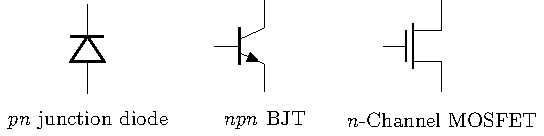
\includegraphics[width=0.8\textwidth]{figure/ch03/fig03-01.pdf}
    \caption{Three most essential electronic components reviewed in this chapter.}
    \label{fig:03-01}
\end{figure}

\section{Basic semiconductor concepts}
Conductivity of a material is proportional the concentration of free electrons.
\begin{equation}
    \begin{split}
    \textbf{Conductor: }\,\, & n_{cond} \approx 10^{28} electrons/m^3 \\
    \textbf{Insulator: }\,\, & n_{ins} \approx 10^{7} electrons/m^3 \\
    \textbf{Semiconductor: }\,\, & n_{ins} < n_{sem} < n_{cond}
    \end{split}
    \label{eq:ch03-elec-conc}
\end{equation}

\subsection{Intrinsic semiconductors}
Silicon or Germanium have crystalline strcuture with four covalent bonds between neighbouring atoms. At $0^\circ K$ semiconductors all covalent bonds are in place tightly holding on to electrons in the bonds. Thus these behave as perfect insulators at low temperatures. With increase in temperature, covalent bonds are ruptured, releasing \textit{free electrons} to roam around in the crystal and become available for conduction when there is an externally applied electric field. The missing electron in the ruptured covalent bond is called a \text{hole}, which too act as carrier of electricity. When an electric field is applied, electrons from neighbouring covalent bonds jump into a hole creating a hole in their previvous bond. This results in the hole effectively moving the direction opposite to the jumping electrons from the covalent bonds. Thus, unlike conductors, semiconductors can have two types of charge carriers: \textit{electrons} and \textit{holes}. The concentration of free electrons and holes in a semiconductor determines it conductivity, which is controlled by temperature. In intrinsic semiconductors, the concentration of free electrons and holes is equal, i.e. $n_{e^-} = n_{h^+} = n_i$. This concentration is given by,
\begin{equation}
    n_i = B \, T^{3/2} \, e^{-\frac{E_g}{k_B T}}
    \label{eq:ch03-intrinsic-elec-conc}
\end{equation}
where $B$ is a material constant ($7.3 \times 10^15 \text{cm}^{-3}\text{K}^{-3/2}$ for Si), $E_g$ is the band gap energy, $k_B$ is the Boltzmann constant, and $T$ is the absolute temperature in Kelvin. The band gap energy is the energy required to break a covalent bond and create a free electron-hole pair. It should be noted that the conductivity of semiconductors increases with temperature, making them suitable for thermometry.

\subsection{Doped Semiconductors}
With intrinsic semiconductors, the conductivity is still quite small at room temperature. Another precise and controlled way to change a semiconductor's conductivity is by adding impurities, called \textit{doping}. The two types of doping are: \textbf{$n$-type} and \textbf{$p$-type} doping. 

In a \textbf{$n$-type} semiconductor, a small amount of pentavalent atoms (e.g. Phosphorus, Arsenic) are added to the semiconductor. These atoms have five valence electrons, and when added to the silicon crystal, four of these electrons form covalent bonds with the neighbouring silicon atoms, while the fifth electron is free to roam around in the crystal. This results in an increase in the concentration of free electrons, making the semiconductor more conductive. The concentration of free electrons in an $n$-type semiconductor is given by,
\begin{equation}
    n_{e^-} = n_i + N_D \quad n_{h^+} = n_i
    \label{eq:ch03-n-type-elec-conc}
\end{equation}
where, $N_D$ is concentration of the doping element.

In a \textbf{$p$-type} semiconductor, a small amount of trivalent atoms (e.g. Boron) is added to the silicon crystal structure. This leaves the dopped elements with four covalent bonds with one of the bonds lacking an electron or a hole. This holes acts as a charge carrier. The concentration of the holes in a $p$-type semiconductor is give by,
\begin{equation}
    n_{h^+} = n_i + N_A \quad n_{e^-} = n_i
    \label{eq:ch03-p-type-elec-conc}
\end{equation}
where, $N_A$ is concentration of the doping element in the $p$-type semiconductor.

The doped semiconductors will have higher conductivity than the intrinsic semiconductors depending on the concentration of the impurities added to the silicon crystal.

\subsection{Flow of current in semiconductors}
There are two types of current flow mechanisms in seminconductors unlike pure conudctors -- (a) \textbf{drift current} and (b) \textbf{diffusion current}. Both are imporant for understanding the operation of the basic electronic components.

\noindent\textbf{Drift current.} Drift current is established by an external electric fields, for examples when a semiconductor is connected to a battery. Holes will accelerate in the direction of the field, while the electrons accelerate in the opposite direction. Bumping into the atoms of the cystral structure, the holes and electrons acquire an average drift velocity given by,
\begin{equation}
    \nu_{p-drift} = \mu_p E \quad \& \quad \nu_{n-drift} = -\mu_n E\
    \label{eq:ch03-drift-vel}
\end{equation}
This constitute a drift current through the semiconductor given by the following,
\begin{equation}
    I_{drift} \propto q\left(n_{h^+}\mu_p + n_{e^-}\mu_n \right) E
    \label{eq:ch03-drift-current}
\end{equation}
where, $q$ is the magnitude of electron charge.

\noindent\textbf{Diffusion current.} Diffusion currents result whena concentration gradient exists across a semiconductor.
\begin{equation}
    I_{diff} \propto -q D_q \frac{d p\left(x\right)}{dx}
    \label{eq:ch03-diff-current}
\end{equation}
where, $p\left(x\right)$ is the concentration of the charge carrier along the $x$ direction. Diffusion currents play an important role in the functioning of the BJT.

\section{Diode}
Whena  $p$-type and $n$-type semiconductors are brought in close contact to each other, there is a big concentration difference between the charge carriers across the interface. A $pn$-junction diode made by bringing a $n$-type and $p$-type semiconductors together as shown in Figure~\ref{fig:03-02}. Due to the concentration difference, electrons from the $n$-type semiconductor diffuse into the $p$-type semiconductor, while holes from the $p$-type semiconductor will diffuse into the $n$-type semiconductor. Note that this is the diffusion current $I_D$, which flows even when the diode is open circuited. This diffusion current sets up the depletion region at the interface, where there are no free charge carriers. This region consists of fixed positive and negative charges, which creates an electric field across the junction. This electric field opposes further diffusion of charge carriers across the junction, and the potential or \textit{barrier voltage} $V_0$ due to the electric field must be overcome for th diffusion current to flow across the junction. Note that the diffusion current $I_D$ is due to the majority charge carriers -- \text{holes} from the $p$ side and \textit{electrons} from the $n$-side.

There is a drift current $I_S$ that flows across the junction due to the minority charge carriers - the \textit{electrons} from the $p$-side and the \textit{holes} from the $n$-side. These thermally generated minority charge carriers, will be swept across and transported across the junction due to the electric field, which tends to reduce the barrier voltage $V_0$. Thus, when the diode is open circuited, we have an equilibrium $I_D = I_S$.

\noindent\textit{Barrier voltage} of a diode depends on several factors, the amount fo doping of the $n$ and $p$ semiconductors, the temperature, etc. The exact relationship is give by,
\begin{equation}
    V_0 = V_T \ln\left(\frac{N_A N_D}{n_i^2}\right)
    \label{eq:ch03-barrier-volt}
\end{equation}
where, $V_T$ is the thermal voltage given by $V_T = \frac{k_B T}{q}$, where $k_B$ is the Boltzmann constant, $T$ is the absolute temperature in Kelvin. For silicon diodes, this is approximately $V_T \approx 26 mV$ at room temperature. The barrier voltage $V_0$ is typically around $0.7 V$ for silicon diodes, and around $0.3 V$ for germanium diodes.

\begin{figure}[t]
    \centering
    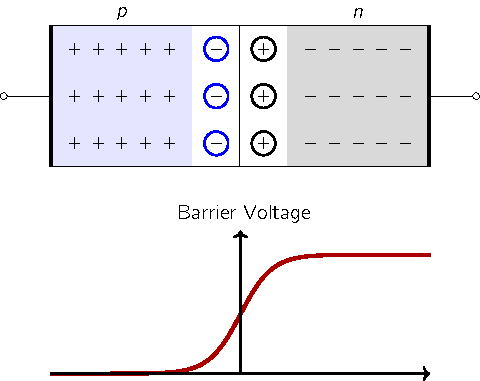
\includegraphics[width=0.6\textwidth]{figure/ch03/fig03-02.pdf}
    \caption{$pn$ junction diode}
    \label{fig:03-02}
\end{figure}

\subsection{Applying a voltage across a diode}
When we connect a voltage source across the diode (Figure~\ref{fig:03-diode-vi}), we can either apply a forward bias or a reverse bias. When the positive terminal of the voltage source is connected to the $p$-side and the negative terminal is connected to the $n$-side, we have a \textbf{forward bias}. This reduces the barrier voltage $V_0$, and allows the diffusion current $I_D$ to flow across the junction. The diode is said to be \textit{on} in this case, and the current $I$ flowing through the diode is called the \textit{forward current}. The voltage-current realtionship between the forward current $I$ and the voltage $V$ across the diode is given by,
\begin{equation}
    I = I_S \left( e^{\frac{V}{V_T}} - 1 \right)
    \label{eq:ch03-forward-bias-vi}
\end{equation}
where, $I_S$ is the saturation current, which is the reverse current that flows when the diode is reverse biased, and , and $q$ is the magnitude of electron charge.

When the negative terminal of the voltage source is connected to the $p$-side and the positive terminal is connected to the $n$-side, we have a \textbf{reverse bias}. This increases the barrier voltage $V_0$, and prevents the diffusion current $I_D$ from flowing across the junction. The diode is said to be \textit{off} in this case, and only a small reverse saturation current $I_S$ flows through the diode.
\begin{figure}[t]
    \centering
    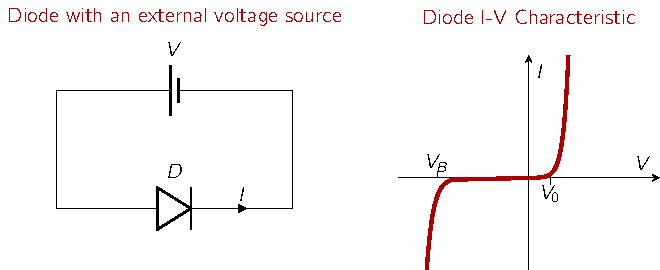
\includegraphics[width=0.7\textwidth]{figure/ch03/fig03-03.pdf}
    \caption{V-I characteristics of a diode}
    \label{fig:03-diode-vi}
\end{figure}
When the reverse biased voltage is increased beyond a certain threshold, called the \textit{breakdown voltage} $V_B$, the diode will start conducting in the reverse direction. This is called \textit{avalanche breakdown}, and the diode can be damaged if the current is not limited by a resistor or some other means. The avalanche breakdown is the reason for the sharp rise in the current at the $V_B$.

\subsection{A simple diode circuit}
\begin{figure}[b]
    \centering
    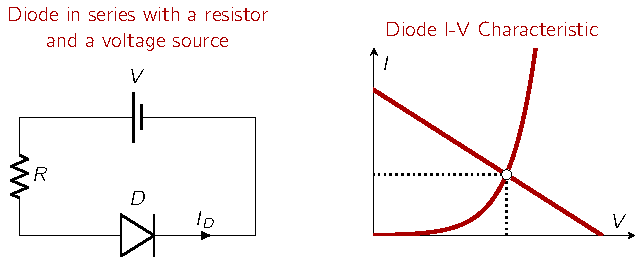
\includegraphics[width=0.7\textwidth]{figure/ch03/fig03-diode-resistor-ckt.pdf}
    \caption{Diode voltage and current in a simple diode circuit with a series resistor.}
    \label{fig:03-diode-resistor-ckt}
\end{figure}
In the circuit shown in Figure~\ref{fig:03-diode-vi}, the moment the forward bias-voltage gets close tot 0.6, the current starts to rise drammatically. Slight changes in the voltage will lead to large changes in the current if it is not limited by a series resistor. Without a resistor, we can easily burn the diode due to large power dissipation across the diode. Consider a more practical cicruit with a voltage source, resistor, and a diode, as shown in Figure~\ref{fig:03-diode-resistor-ckt}. The voltage across the diode $V_D$ and the current through the diode $I_D$ by writing the Kirchoff voltage law (KVL) around the loop,
\begin{equation}
    V - I_D R - V_D = 0
    \label{eq:ch03-diode-resistor-kvl}
\end{equation}
The current $I_D$ and $V_D$ from Eq.~\ref{eq:ch03-forward-bias-vi} can be substituted into Eq.~\ref{eq:ch03-diode-resistor-kvl} to solve for $V_D$ and $I_D$,
\begin{figure}[t]
    \centering
    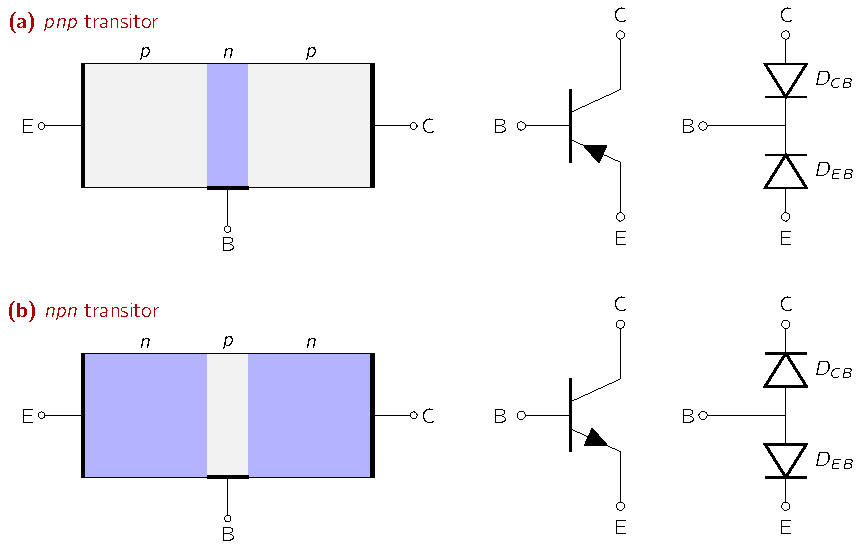
\includegraphics[width=0.8\textwidth]{figure/ch03/fig03-bjt-struct.pdf}
    \caption{Bipolar junction transistor structure and symbol}
    \label{fig:03-04}
\end{figure}
\begin{equation}
    V - R I_S \left( e^{\frac{V_D}{V_T}} - 1 \right) - V_D = 0
    \label{eq:ch03-diode-resistor-vd-id}
\end{equation}
Unfortunately, this is a non-linear solution will need to be solved to find the voltage across the diode $V_D$ and the current through the diode $I_D$. 

Let's assume that $V=5V$ and $R=1k\Omega$ in Figure~\ref{fig:03-diode-resistor-ckt}. A first order approximation can be made by assuming that the diode is \textit{switched off}, i.e. no current is flow through it and see if it leads to a contradiction. If we assume the diode is off and no current is flowing $I_D = 0mA$ through it, then $V_D = 5V$ The diode cannot be off if $V_D \geq 0.7V$. So, the diode must be swtiched on. We will assume that the diode is on and then find out the current flowing through it and check that it is not close to 0. In the current circuit, have 
\begin{equation}
    I_D \approx \frac{V - 0.7}{R} = 4.3mA
    \label{eq:ch03-diode-resistor-id-approx}
\end{equation}
$I_D$ is large enough for to flow through the didode when its switched on. Thus, $V_D=0.7V$ and $I_D=4.3mA$ is a reasonable first approximation of the diode's voltage and current in the current circuit.

\section{Bipolar junction transistor (BJT)}
The bipolar junction transistor (BJT) is the first of some of the three terminal devices we will come across int his course. There are two types of BJTs -- $npn$ and $pnp$. BJTs are formed by sandwiching a thin layer of $p$-type semiconductor between two $n$-type semiconductors or vice versa. This is depicted in Figure~\ref{fig:03-04}. Metal contacts are made with these three semiconductor regions to form the three terminals of the BJT. In an $npn$ BJT, one of the  $n$ regions is the \textit{emitter} which is heavily dopped, and the other $n$ region is the \textit{collector}. The $p$ region is the \textit{base}, which is lightly doped and very thin compared to the widths of the emitter and collector regions. The collector is moderately doped. Three terminal devices like the BJT and MOSFET can be used as an amplifier or a switch, depending on how it is biased. We will only discuss $npn$ transistors for the rest of the section; the $pnp$ transistor is similar, but with the polarities of the voltages and currents reversed.A BJT is essentially two diodes connected back to back as shown in Figure~\ref{fig:03-04}

A BJT can be operated in three different modes, depending on the biasing of the terminals. The three modes are: (a) \textbf{Cut-off mode}, (b) \textbf{Active mode}, and (c) \textbf{Saturation mode}. The difference between the three modes are summarized in Table~\ref{tab:03-bjt-modes}.
\subsection{Cut-off mode}
In this mode, the emitter-base (EB) and the collector-base (CB) junctions are reverse biased, and not current flows through the transistor.
\begin{equation}
    I_E = 0 \quad I_B = 0 \quad I_C = 0
    \label{eq:03-bjt-cutoff}
\end{equation}
\subsection{Active mode}
In this mode, the EB junction is forward biased, while the CB junction is reverse biased. Consider the circuit in Fig.~\ref{fig:03-bjt-active}.
\begin{figure}[h]
    \centering
    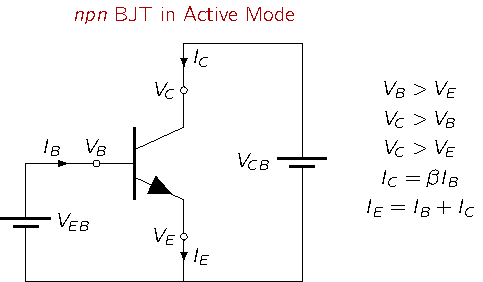
\includegraphics[width=0.55\textwidth]{figure/ch03/fig03-bjt-active.pdf}
    \caption{$npn$ BJT in active mode.}
    \label{fig:03-bjt-active}
\end{figure}
When the $npn$ BJT's EB junction is forward biased ($V_{BE} \approx 0.7V$), electrons (the majority carrier) from the highly doped emitter region are injected just across the EB junction. The electrons diffuse into the base region, which is lighly doped and very thin. Because $V_C > V_B$, the injected electrons are swept across the base region by the electric field created by the reverse biased CB junction. A small percentage of these injected electrons recombibe with the holes in the base region, which contributes to the small base current. The collector current will be proportional the base current; the current gain is given by the parameter $\beta$.
\begin{equation}
    I_C = \beta I_B \quad \text{where, } \beta \approx 100 - 1000
    \label{eq:03-bjt-active-ic}
\end{equation}
An equivalent circuit of the BJT in the active model is shown in the following figure (Fig.~\ref{fig:03-bjt-active-eqt}). In this circuit, assume that the supply voaltges $V_{BB}$, $V_{CC}$, and the resistors $R_B$ and $R_C$ are chosen appropriately to place the $npn$ transistor in the active mode. The AC source $v_{s}$ of sufficiently small in amplitude (in $mV$) will result in small changes in $I_B$, which lead to corresponding change in $I_C$. The voltage at the collector $V_C$ have a larger amplitude variations riding on a DC voltage, given by the following,
\begin{equation}
    V_C = V_{CC} - \beta \frac{R_C}{R_B}\left(V_{BB} - 0.7 \right) -  \beta \frac{R_C}{R_B} v_s
    \label{eq:03-bjt-active-vc}
\end{equation}
This is easy to derive and is left as an exercise for the reader. The input voltage $v_s$ get amplified by a factor of $\beta \frac{R_C}{R_B}$, which is the voltage gain of this the common emitter amplifier circuit. We will no disucss such circuits any further in the course. This was just to illustrate the utility of the BJT in amplifying small AC signals when operated in the active mode.
\begin{table}[h]
    \centering
    \caption{Modes of operation of a bipolar junction transistor (BJT)}
    \begin{tabular}{ c c c l}
    \hline
    \rowcolor[HTML]{F8F8F8} 
    \textbf{Mode} &
    \textbf{\begin{tabular}[c]{@{}c@{}}Emitter-Base\\ Junction\end{tabular}} &
    \textbf{\begin{tabular}[c]{@{}c@{}}Collector-Base\\ Junction\end{tabular}} &
    \multicolumn{1}{c}{\textbf{Operation}} \\ \hline
    Cut-off &
    Reverse biased &
    Reverse biased &
    Transistor is off; no current flows. \\ \hline
    Active &
    Forward biased &
    Reverse biased &
    $I_C$ is proportional to $I_B$ \\ \hline
    Saturation &
    Foward biased &
    Forward biased &
    $I_C$ and $V_{CE}$ saturate. \\ \hline
    \end{tabular}
    \label{tab:03-bjt-modes}
\end{table}

\subsection{Saturation mode}
Consider the circuit in Fig.~\ref{fig:03-bjt-sat-eqt}. If for fixed $V_{BB}$, we reduce $R_B$, this will increase $I_B$, which would result in progressively increasing $I_C$. However, $I_C$ cannot continue to increase forever. As $I_C$ increases, $V_C = V_{CC} - I_{C}R_{C}$ decreases. Once its value falls sufficiently below the base voltage $V_B$, the collector-base (CB) junction becomes forward biased. This is called the \textbf{saturation mode} of operation of the BJT. In this mode, the BJT behaves like a closed switch, and the collector current $I_C$ saturates at a value that is independent of the base current $I_B$. The collector-emitter voltage saturates at $V_{CE(sat)} \approx 0.2V$ for silicon BJTs, making the collector current independent of the base current.
\begin{figure}[t]
    \centering
    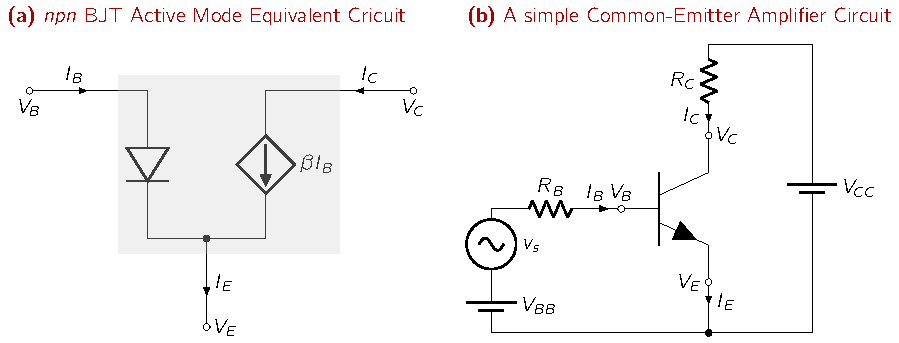
\includegraphics[width=\textwidth]{figure/ch03/fig03-bjt-active-eq.pdf}
    \caption{$npn$ BJT active mode equivalent circuit, and a simple common emitter voltage amplifier circuit.}
    \label{fig:03-bjt-active-eqt}
\end{figure}
\begin{equation}
    I_C \approx \frac{V_{CC} - V_{CE(sat)}}{R_C} \quad \text{and } V_{CE(sat)} \approx 0.2V
    \label{eq:03-bjt-sat-ic}
\end{equation}
The saturation mode is used in switching applications, where the BJT is used as a switch to turn on or off a load connected to the collector; think of the collector resistor as the load. We will discuss some applications later in the chapter.

\begin{figure}[b]
    \centering
    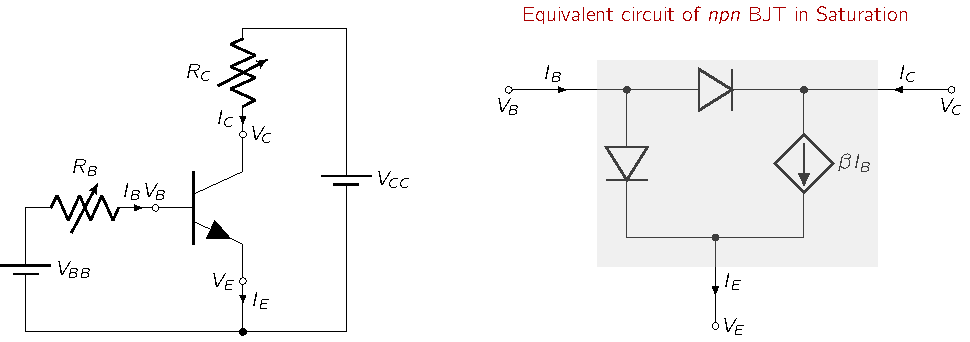
\includegraphics[width=\textwidth]{figure/ch03/fig03-bjt-sat-eq.pdf}
    \caption{$npn$ BJT active mode equivalent circuit, and a simple common emitter voltage amplifier circuit.}
    \label{fig:03-bjt-sat-eqt}
\end{figure}

\section{Metal oxide field effect transistor (MOSFET)}
While the BJT might be a popular choice for many applications where circuits are made on a breadboard or a PCB. However, when it comes to integrated circuits, the MOSFET is the most popular choice. MOSFETS can be made quite small, are easier to fabricate, and consume less power than BJTs. They canb be use for both digitial and analog integrated circuits. There are four types of MOSFETs, $n$-channel or $p$-channel textit{enhancement} or \textit{depeltion} type MOSFETs. In this section, we will only focus on the enhancement-type $n$-channel MOSFET to understand the fundamental principle of operation of the MOSFETs.

\begin{figure}[t]
    \centering
    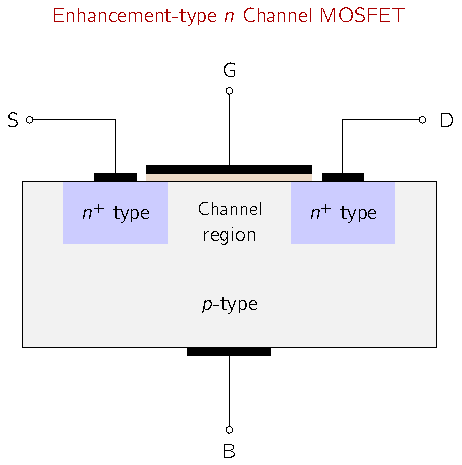
\includegraphics[width=0.45\textwidth]{figure/ch03/fig03-mosfet-struct.pdf}
    \caption{$n$ Channel Enhancement MOSFET.}
    \label{fig:03-mosfet-struct}
\end{figure}

The physical structure of an enhancement-type $n$-channel MOSFET is shown in Figure~\ref{fig:03-mosfet-struct}. The MOSFET in this figure has four terminals - source (S), drain (D), gate (G), adn body (B). The source and drain are heavily doped $n$-type regions, while the channel is lightly doped $p$-type region. The region between drain and the source is called the \textit{channel region}. The gate is insulated from the channel by a thin layer of oxide, which acts as a dielectric. The gate terminal is used to control the formation of a conductive channel between the source and drain terminals. The body terminal is connected to the source terminal, and is usually shorted to the source in most applications. The MOSFET is a four terminal device, but it can be treated as a three terminal device by shorting the body and source terminals.

The drain is always kept at then higher potential than then source. The connection between the drain to the source is essentially two diodes connected back-to-back, implying that applying a voltage between the drain and source does not result in any current because one of the diodes if reverse biased. However, when a positive voltage is applied to the gate with respect to the body/source, things get interesting as shown in Figure~\ref{fig:03-mosfet-gate-volt}. Applying a positive gate voltage $V_{GS}$ with respect to the source terminal creates an electric field across the oxide layer, which penetrates into the channel region. This electric field attracts electrons in to the channel region right below the gate oxide layer. As the voltage in increased beyond a threshold $V_t$, a conductive channel is formed between the source and drain terminals, which can now conduct current between the source and the drain. The threshold voltage is typically between $0.3V-1.0V$. Any $v_{GS}$ applied beyond $V_t$ is called the \text{overdrive} votlage or \textit{effective} voltage $v_{OV}$.

\begin{figure}[t]
    \centering
    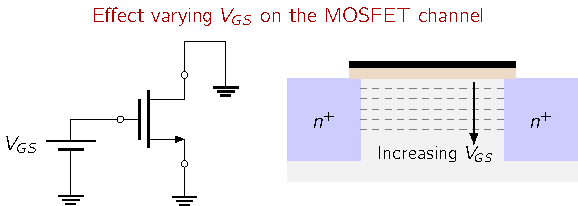
\includegraphics[width=0.8\textwidth]{figure/ch03/fig03-mosfet-vgs-vds.pdf}
    \caption{$n$-Channel MOSFET $V_{GS}$-$V_{DS}$ Characteristics.}
    \label{fig:03-mosfet-gate-volt}
\end{figure}

In Figure~\ref{fig:03-mosfet-gate-volt} no current flows because both the source and drain are grouded. When a drain source voltage is applied, as shown in Figure~\ref{fig:03-mosfet-drainsource-volt}, the MOSFET can be turned on by applying a positive gate voltage $V_{GS}$ with respect to the source. The current flowing through the MOSFET is called the \textit{drain current} $I_D$. The relationship between the drain current $i_D$, the gate-source voltage $V_{GS}$, and the drain-source voltage $V_{DS}$ is given by,
\begin{equation}
    i_D = k_n\left(\left(v_{GS} - V_t\right)v_{DS} - \frac{1}{2}v_{DS}^2\right)
    \label{eq03-mosfet-id-vgs}
\end{equation}
where, $k_n$ is the process transconductance parameter, and $V_t$ is the threshold voltage. This expression hold only when $V_{GS} > V_t$ and $0 \leq V_{DS} < V_{GS} - V_t$. Something very interesting happens to the channel when a drain-source voltage is applied and its magnitude is increased, as shown in Figure~\ref{fig:03-mosfet-vds-pinchoff}. The channel becomes trapizoidal in shape as $v_{DS}$ is increased due to different is $g_{GS}$ and $v_{GD}$. This causes the resistance of the channel to increase, tapering off the current flowing through it. When the $v_{DS}$ is increased further, the channels gets pinched off and the current saturates.
\begin{figure}[b]
    \centering
    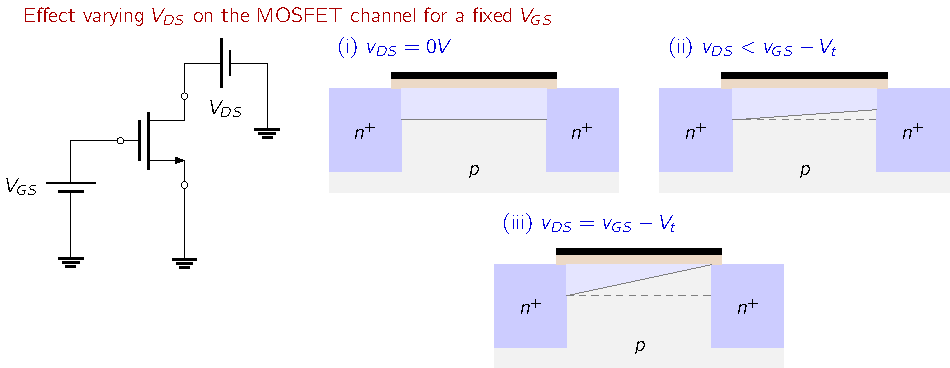
\includegraphics[width=1\textwidth]{figure/ch03/fig03-mosfet-vds-pinchoff.pdf}
    \caption{$n$-Channel MOSFET $V_{DS}$ Characteristics.}
    \label{fig:03-mosfet-vds-pinchoff}
\end{figure}

\subsubsection{MOSFET regions of operation}
The MOSFET can bwe operated in three different regions, depending on the values of $V_{GS}$ and $V_{DS}$. The three regions are: (a) \textbf{Cut-off region}, (b) \textbf{Triode region}, and (c) \textbf{Saturation region}. The difference between the three regions are summarized in Table~\ref{tab:03-mosfet-regions}.

\begin{table}[h]
    \centering
    \caption{Modes of operation of a MOSFET}
    \begin{tabular}{ c c c l}
    \hline
    \rowcolor[HTML]{F8F8F8} 
    \textbf{Mode} &
    \textbf{\begin{tabular}[c]{@{}c@{}}Gate-Source\\ Voltage\end{tabular}} &
    \textbf{\begin{tabular}[c]{@{}c@{}}Drain-Source\\ Voltage\end{tabular}} &
    \multicolumn{1}{c}{\textbf{Operation}} \\ \hline
    Cut-off &
    $V_{GS} < V_t$ &
    $V_{DS} = 0$ &
    Transistor is off; no current flows. \\ \hline
    Triode &
    $V_{GS} > V_t$ &
    $V_{DS} < V_{GS} - V_t$ &
    $I_D$ is proportional to $V_{DS}$. \\ \hline
    Saturation &
    $V_{GS} > V_t$ &
    $V_{DS} \geq V_{GS} - V_t$ &
    $I_D$ is constant. \\ \hline
    \end{tabular}
    \label{tab:03-mosfet-regions}
\end{table}

% \noindent\textbf{Independent Voltage source.} An idea voltage source provides a fixed voltage $V$ between its two terminals, and can provide any amount of current. Notice that the voltage $V$ can be fixed or time varying. For example, for a DC vortlage source with $V = 5V$, the voltage across the two terminals will be $5V$ for all time. But for a time varying AC source, $V = 5 \sin \left( 100\pi t \right)$, the voltage across its terminal will vary with time. We will often drop the adjective "independent" when we are sure that the context is clear. We will look at dependent sources later, and we will always use the adjective "dependent" to refer to them.

% \noindent \textbf{Independent Current source.} An ideal cuyrrent source provide a fixed amount of current to flow throgh its terminals (out through one and in through the other), irrespective of the voltage across its terminals. Current sources can also be time-varying.

% \noindent \textbf{Resistor.} A passive element where the current $i_R$ flowing through the element is proportional to the voltage $v_R$ across its terminals.
% \[ v_R \propto i_R \]
% In the case of linear resistors, the proportionality factor is constant, resulting in Ohm's law,
% \begin{equation}
%     v_R = R \, i_R
%     \label{eq:02-01}
% \end{equation}

% The units of $R$ are $V.A^{-1}$ or $Omhs \left( \Omega \right)$. $R$ is in general positive. The power absorbed by a resistor is given by the product of the voltage across it and the current flowing through the resistor, 
% \begin{equation}
%     P = v_R \, i_R = i_R^2 \, R = \frac{v_R^2}{R}
%     \label{eq:02-02}
% \end{equation}
% This power is dissipated as heat by the resistor. Note that the power absorbed by a resistor is always positive, since $R$ is positive.

% We will later see non-linear resistors, where the resistance varies as a function of the applied votlage, temperature and other factors. 

% \noindent \textbf{Capacitor.} A capacitor is another passive element with the following voltage current relationship.
% \begin{equation}
%     i_C = C \frac{d v_C}{dt}
%     \label{eq:02-03}
% \end{equation}

% The current $i_C$ through the capacitor is proportional to the rate of change of voltage across its terminals $v_C$. The proportionality factor is called the capacitance $C$, and has units of $F$ (Farads) or $C \cdot V^{-1}$. The voltage across the capacitor is given by at any given time is proportional to the integral of the current flowing through itor the charge stored in the capacitor. The voltage across the capacitor is given by
% \begin{equation}
%     q = C \, v_C
%     \label{eq:02-04}
% \end{equation}

% The instantaneous power absorbed by the capacitor is given by,
% \begin{equation}
%     P = v_C \, i_C = C \, v_C \frac{d v_C}{dt}
%     \label{eq:02-05}
% \end{equation}

% The power absorbed by the capacitor can be positive or negative, depending on the direction of current flow. If the current is flowing into the capacitor, then the voltage across it is increasing, and the power absorbed is positive. If the current is flowing out of the capacitor, then the voltage across it is decreasing, and the power absorbed is negative. A capacitor stores energy in the electric field between its plates. The energy stored in a capacitance at any given time depends on the charge stored in it, and is given by,
% \begin{equation}
%     E = \frac{1}{2}  C \, v_C^2
%     \label{eq:02-06}
% \end{equation}

% \noindent \textbf{Inductor.} An inductor is another passive element with the following voltage current relationship.
% \begin{equation}
%     v_L = L \frac{di_L}{dt}
%     \label{eq:02-07}
% \end{equation}

% The voltage $v_L$ across the inductor is proportional to the rate of change of current $i_L$ flowing through it. The proportionality factor is called the inductance $L$, and has units of $H$ (Henries) or $V \cdot s \cdot A^{-1}$. The current through the inductor is given by at any given time is proportional to the integral of the voltage across it. The current through the inductor is given by
% \begin{equation}
%     i_L = \frac{1}{L} \int v_L \, dt
%     \label{eq:02-08}
% \end{equation}

% The instantaneous power absorbed by the inductor is given by,
% \begin{equation}
%     P = v_L \, i_L = L \, i_L \frac{di_L}{dt}
%     \label{eq:02-09}
% \end{equation}

% The power absorbed by the inductor can be positive or negative, depending on the direction of current flow. If the current is flowing into the inductor, then the voltage across it is increasing, and the power absorbed is positive. If the current is flowing out of the inductor, then the voltage across it is decreasing, and the power absorbed is negative. An inductor stores energy in the magnetic field around it. The energy stored in an inductor at any given time depends on the current flowing through it, and is given by,
% \begin{equation}
%     E = \frac{1}{2}  L \, i_L^2
%     \label{eq:02-10}
% \end{equation}

% \subsection{Kirchoff's Laws}
% The five elements alone are not that interesting. But interesting things can be done by connecting these elements together in different ways to form an electrical circuit. The elements are connected together by wires, whicha are assumed to be perfect conductors, i.e. zero resistance. Consider the following circuit (Figure \ref{fig:02-01}),
% \begin{figure}[t]
%     \centering
%     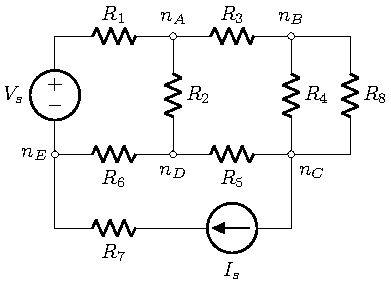
\includegraphics[width=0.5\textwidth]{figure/ch02/fig02-02.pdf}
%     \caption{A simple electrical circuit with a voltage sourse, a current source, and a bunch of resistors.}
%     \label{fig:02-02}
% \end{figure}

% How do we find out the voltages and currents in the circuit? Kirchoff's laws can be used for analysing such circuits, which are based on the conservation of charge and energy. The circuit in Figure \ref{fig:02-02} is a simple electrical circuit with a voltage source, a current source, and a bunch of resistors. The voltage source provides a fixed voltage $V_s$ between its two terminals, and the current source provides a fixed amount of current $I_s$ to flow through its terminals. The voltages and currents in the rest of the elements will be determined by Kirchoff's laws with the constraints imposed by the voltage and current sources. The two laws are:

% \begin{enumerate}
%     \item \textbf{Kirchoff's current law (KCL):} The sum of the currents entering a node is equal to the sum of the currents leaving the node. A \textit{node} is a point at which two or more circuit elements are connected together. In Figure \ref{fig:02-02}, $n_A$, $n_B$, $n_C$ and $n_D$ are examples of nodes where three elements are connected together. There are three other nodes in the circuit, can you identify them? 
    
%     The sum of the currents at a node is equal to zero. This is based on the conservation of charge, and can be expressed mathematically as:
%     \begin{equation}
%         \sum_{i=1}^{n} i_i = 0
%         \label{eq:02-11}
%     \end{equation}
%     where $i_i$ is the current flowing into or out of the node, and $n$ is the number of elements connected to the node. The current flowing into a node is positive, and the current flowing out of a node is negative.
    
%     \item \textbf{Kirchoff's voltage law (KVL):} The sum of the voltages around a closed loop in a circuit is equal to zero. A \textit{closed loop} is a path in the circuit that starts and ends at the same node, and does not cross itself. In Figure \ref{fig:02-02}, the path starting from $n_A$, to $n_D$, to $n_B$, and back to $n_A$ is a closed path. This path invludes the resistors $R_3$, $R_4$, $R_5$, and $R_2$. 
    
%     This is based on the conservation of energy, and can be expressed mathematically as:
%     \begin{equation}
%         \sum_{i=1}^{n} v_i = 0
%         \label{eq:02-12}
%     \end{equation}
%     where $v_i$ is the voltage across each element in the loop, and $n$ is the number of elements in the loop.

%     The voltage across an element is positive if the current is flowing into the positive terminal of the element, and negative if the current is flowing out of the positive terminal of the element.
% \end{enumerate}

% Note that the two laws apply for any type of circuit element used in the circuits, independnet or dependent voltage/current sources, resistors, capacitors, inductors, other two, three or four terminal elements.

% \subsection{Series and Parallel Connections}
% Two elements that share the same voltage across them between a given pair of notes are said to be \textbf{parallel} to each other. In Figure~\ref{fig:02-02}, $R_4$ and $R_8$ are parallel to each other. In a single loop, two elements that share the same current are said to be in \textbf{series} with each other. In Figure~\ref{fig:02-02}, $V_s$ and $R_1$ are in series, $I_s$ and $R_7$ are in series.

% \subsubsection{Resistors in series and parallel}
% When $n$ resistors $R_1, R_2, \cdots R_n \geq 0$ are in series, these can be combined to an equivalent resistor with resistance $R_{eq}$ given by the following,
% \begin{equation}
%     R_{eq} = \sum_{i=1}^{n} R_i \implies R_{eq} \geq \max_{1 \leq i \leq n} R_i.
%     \label{eq:02-13}
% \end{equation}
% Note that in a series connection the equivalent resistance is at least as large as the largest value of $R_1$ to $R_n$.

% When $n$ resistors $R_1, R_2, \cdots R_n \geq 0$ are in parallel, these can be combined to an equivalent resistor with resistance $R_{eq}$ given by the following,
% \begin{equation}
%     \frac{1}{R_{eq}} = \sum_{i=1}^{n} \frac{1}{R_i} \implies R_{eq} = \frac{R_1R_2\cdots R_n}{R_1 + R_2 + \cdots + R_n} \implies R_{eq} \leq \min_{1 \leq i \leq n} R_i
%     \label{eq:02-14}
% \end{equation}
% Note that in a parallel connection, the equivalent resistance cannot be larger than the smallest value of $R_1$ to $R_n$.

% \subsubsection{Capacitors in series and parallel}
% \noindent\textbf{Series connection} of $n$ capacitors $C_1, C_2, \cdots C_n \geq 0$
% \begin{equation}
%     C_{eq} = \frac{C_1C_2\cdots C_n}{C_1 + C_2 + \cdots + C_n}
%     \label{eq:02-15}
% \end{equation}

% \noindent\textbf{Parallel connection} of $n$ capacitors $C_1, C_2, \cdots C_n \geq 0$
% \begin{equation}
%     C_{eq} = C_1 + C_2 + \cdots + C_n
%     \label{eq:02-16}
% \end{equation}

% \subsubsection{Inductors in series and parallel}
% \noindent\textbf{Series connection} of $n$ capacitors $L_1, L_2, \cdots L_n \geq 0$
% \begin{equation}
%     L_{eq} = L_1 + L_2 + \cdots + L_n
%     \label{eq:02-17}
% \end{equation}

% \noindent\textbf{Parallel connection} of $n$ capacitors $L_1, L_2, \cdots L_n \geq 0$
% \begin{equation}
%     L_{eq} = \frac{L_1L_2\cdots L_n}{L_1 + L_2 + \cdots + L_n}
%     \label{eq:02-18}
% \end{equation}
% Its left as an exercise for you to verify these expressions.

% \noindent\textbf{What does the equivalent resistance actually mean?} The equilvant resistor with resistance $R_{eq}$ has the same voltage-current relationship as the individual elements in series or parallel connection. We can replace the series or parallel connection of the individual resistors $R_1$ to $R_n$ by a single resistor with value $R_{eq}$ without changing the volatage current relationships in the circuit. The same argument applies for equivalent capacitors and inductors.

% \subsubsection{Voltage sources in series and parallel}
% \noindent\textbf{Series connection} of $n$ voltage sources $V_1, V_2, \cdots V_n$ will result in an equivalent voltage source $V_{eq}$ given by
% \begin{equation}
%     V_{eq} = V_1 + V_2 + \cdots + V_n
%     \label{eq:02-19}
% \end{equation}
% Voltage soruces should not be connected in parallel, as this will result in a short circuit. Ideally, an infinite currelt will flow through the connection, because the volaage sources force a potential difference between the two end of the wires and it has zero resistance. Parallel connections are allowed only when the two sources have the same voltage and polarity.

% \subsubsection{Current sources in series and parallel}
% \noindent\textbf{Parallel connection} of $n$ current sources $I_1, I_2, \cdots I_n$ will
% result in an equivalent current source $I_{eq}$ given by
% \begin{equation}
%     I_{eq} = I_1 + I_2 + \cdots + I_n
%     \label{eq:02-20}
% \end{equation}
% Current sources should not be connected in series; series connections are allowed only when the two sources have the same current and polarity.

% \subsection{Superposition Principle}
% Linear approximations of circuits are often employed as first order approximations when analysing circuits. A linear ciruit is one that consists of linear passive elements, independent sources and linear dependent sources. Linear circuits follow the superposition principle, which states that the response of a linear circuit to a linear combination of inputs is equal to the corresponding linear comibnation of the responses to each input applied separately. Solving the following circuit (Figure~\ref{fig:02-03}) should make this concept clear.
% \begin{figure}[t]
%     \centering
%     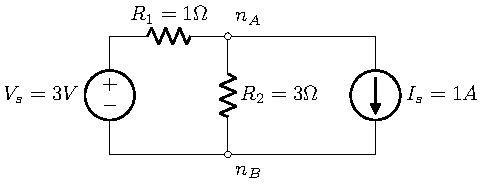
\includegraphics[width=0.65\textwidth]{figure/ch02/fig02-03.pdf}
%     \caption{A simple circuit with two sourcers}
%     \label{fig:02-03}
% \end{figure}
% For the circuit in Figure~\ref{fig:02-03}, perform the following calculation and compare your results.

% \noindent\textbf{Step 1.} Solve for the voltage across and the current through the resistors $R_1$ and $R_2$; we will refer to these are $v_{R1}, i_{R1}$ and $v_{R2}, i_{R2}$, respectively. You should use both Kirchoff's current and voltages laws to compute these variables.

% \noindent Let's now consider of the sources in the circuit seperately. This would mean making the source values ``zero''. This corresponds to two different operations on the circuit. Zeroing a voltage source corresponds to replacing it with a wire (a short circuit), while zeroing a current source corresponds to simple removing the current source (an open circuit). 

% \noindent\textbf{Step 2.} Zero the voltage source $V_s$ and compute the voltages and currents associated with the two resistors. We will refer to these as $v_{R1,V_s=0}$, $v_{R2,V_s=0}$, $i_{R1,V_s=0}$, and $i_{R2,V_s=0}$.

% \noindent\textbf{Step 3.} Zero the current source $I_s$ and compute the voltages and currents associated with the two resistors. We will refer to these as $v_{R1,I_s=0}$, $v_{R2,I_s=0}$, $i_{R1,I_s=0}$, and $i_{R2,I_s=0}$.

% \noindent\textbf{Step 4.} For a linear circuit, shown in Figure~\ref{fig:02-03}, the following will always be true.
% \begin{equation}
%     \begin{split}
%         v_{R1} &= v_{R1,V_s=0} + v_{R1,I_s=0}\\
%         v_{R2} &= v_{R2,V_s=0} + v_{R2,I_s=0}\\
%         i_{R1} &= i_{R1,i_s=0} + i_{R1,I_s=0}\\
%         i_{R2} &= i_{R2,i_s=0} + i_{R2,I_s=0}\\
%     \end{split}
%     \label{eq:02-21}
% \end{equation}

% \noindent Let's assume that I am only interested in $i_{R2}$. Can I use $i_{R2,V_s=0}$ and $i_{R2,I_s=0}$ to compute the current $i_{R2}$ if $V_s = 1V$ and $I_s=-2A$? 

% \subsection{Practical Voltage and Current Sources}
% The independent voltage and current sources we have discussed so far are ``ideal'' sources. Practical or real sources do not behave like them - a battery cannot provide any amount of current for a load without any changes to the voltage across its terminals.

% A good model of practical voltage source is an ideal voltage source $V_s$ in series with a \textit{internal}, \textit{source} or \textit{output} resistor $R_s$. And for a practical current source, it is an ideal current source $I_s$ in parallel with a resistor $R_s$. The voltage across the terminal of a voltage source as function of the current draw from it is depicted for an ideal and practical voltage source in Figure~\ref{fig:02-04}. For the ideal source (Figure~\ref{fig:02-04a}), the voltage $v_L$ is independent of the current $i_L$ drawn from it. For the practical voltage source (Figure~\ref{fig:02-04b}), the voltage across the terminals is a function of the current drawn from it,
% \begin{equation}
%     v_L = V_s - R_s \, i_L
%     \label{eq:02-22}
% \end{equation}
% When $R_L = \infty$ ($i_L = 0$), the voltage across the terminals is equal to the voltage of the source $V_s$. This is maximum voltage the practical source can provide. This is also know as the \textit{open circuit voltage} $v_{oc}$ of the source. When $R_L = 0$ ($v_L = 0$), the current drawn from the source $i_L = \frac{V_s}{R_s}$. This is the maximum current the voltage source can provide. This is also known as the \textit{short circuit current} $i_{sc}$ of the source.

% \begin{figure}[t]
%     \centering
%     \begin{subfigure}{0.48\textwidth}
%         \centering
%         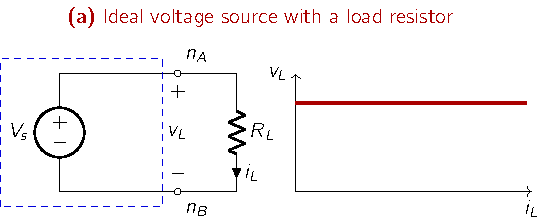
\includegraphics[width=\textwidth]{figure/ch02/fig02-04a.pdf}
%         \caption{Ideal voltage source}
%         \label{fig:02-04a}
%     \end{subfigure}
%     \hfill
%     \begin{subfigure}{0.48\textwidth}
%         \centering
%         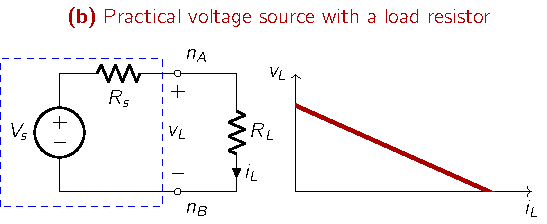
\includegraphics[width=\textwidth]{figure/ch02/fig02-04b.pdf}
%         \caption{Practical voltage source with a load}
%         \label{fig:02-04b}
%     \end{subfigure}
%     \caption{Comparison of the voltage-current relationship of an ideal and a practical voltage source.}
%     \label{fig:02-04}
% \end{figure}

% \begin{boxedstuff}
%     \begin{problem}
%         Plot the voltage-current relationship of a practical current source with $I_s = 2A$ and $R_s = 10\Omega$. What are $v_{oc}$ and $i_{sc}$?
%     \end{problem}
% \end{boxedstuff}

% \subsection{Thevenin's and Norton's Theorems}
% Thevenin's and Norton's theorems are two important theorems in circuit theory that allow us to simplify complex circuits into simpler equivalent circuits. These theorems are based on the superposition principle, and can be used to analyze linear circuits with independent and dependent sources.

% \noindent\textbf{Thevenin's Theorem.} Thevenin's theorem states that any linear circuit with independent and dependent sources can be replaced by an equivalent circuit with a single voltage source $V_{th}$ in series with a resistor $R_{th}$, connected to the load resistor $R_L$. 

% \noindent\textbf{Norton's Theorem.} Norton's theorem states that any linear circuit with independent and dependent sources can be replaced by an equivalent circuit with a single current source $I_{N}$ in parallel with a resistor $R_{N}$, connected to the load resistor $R_L$.
% \begin{figure}[t]
%     \centering
%     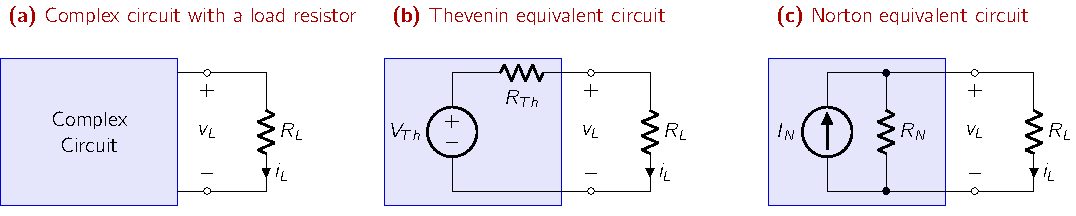
\includegraphics[width=\textwidth]{figure/ch02/fig02-05.pdf}
%     \caption{Thevenin's and Norton's circuits for a complex linear circuit. The Thevenin and Norton equivalent circuits have the same voltage-current relationship for any load.}
%     \label{fig:02-05}
% \end{figure}

% \noindent\textbf{Computing the Thevenin and Norton equivalent circuits.} The Thevenin and Norton equivalent circuits can be computed using the following steps:
% \begin{enumerate}
%     \item Remove the load resistor $R_L$ from the circuit.
%     \item Compute the open circuit voltage $v_{oc}$ across the terminals of the load resistor. This is the Thevenin voltage $V_{th}$. This can be using the superposition principle, where we zero all the independent sources except one and compute the open circuit voltage. The overall open circuit voltage is the sum of the open circuit voltages when all other sources are zeroed.
%     \item Compute the short circuit current $i_{sc}$ through the terminals of the load resistor. This is the Norton current $I_{N}$. This too can be calculated using the superposition principle.
%     \item Compute the Thevenin resistance $R_{th}$ by zeroing all independent sources in the circuit and computing the equivalent resistance seen from the terminals of the load resistor (without the load resistor). This is also equal to the Norton resistance $R_{N}$.
%     \item The Thevenin and Norton equivalent circuits are then given by:
%     \begin{equation}
%         \begin{split}
%             V_{th} &= v_{oc}\\
%             I_{N} &= i_{sc}\\
%             R_{th} &= R_{N}
%         \end{split}
%         \label{eq:02-23}
%     \end{equation}
%     \item The load resistor $R_L$ can be connected to either the Thevenin or Norton equivalent circuit, and the voltage and current across it can be computed using the voltage-current relationship of the equivalent circuit.
% \end{enumerate}

% \begin{boxedstuff}
%     \begin{problem}
%         Compute the Thevenin and Norton equivalent circuits for the circuit shown in Figur~\ref{fig:02-02} assuming the following as the load resistor: (a) $R_8$; (b) $R_2$; and (c) $R_7$.
%     \end{problem}
% \end{boxedstuff}

% \subsection{Maximum Power Transfer Theorem}
% The maximum power transfer theorem states that the maximum power is transferred to the load resistor $R_L$ when the load resistance is equal to the Thevenin resistance $R_{th}$ of the circuit. Consider the following circuit (Figure~\ref{fig:02-06}). The power absorbed by the load resistor $R_L$ is given by,
% \begin{equation}
%     P_{R_L} = \frac{R_L}{(R_{th} + R_L)^2} \, V_{th}^2
%     \label{eq:02-24}
% \end{equation}
% Its easy to check that the optimal value of $R_L$ that maximizes the power absorbed by the load resistor is given by,
% \begin{equation}
%     \begin{split}
%         R_L^* &= \arg\max_{R_L} \,\, \frac{R_L}{(R_{th} + R_L)^2} \, V_{th}^2 = R_{Th} \\
%         P_L^* &= \max_{R_L} \,\, \frac{R_L}{(R_{th} + R_L)^2} \, V_{th}^2 = \frac{1}{4}\left(\frac{V_{Th}^2}{R_{Th}}\right)
%     \end{split}
%     \label{eq:02-25}
% \end{equation}

% \begin{figure}[t]
%     \centering
%     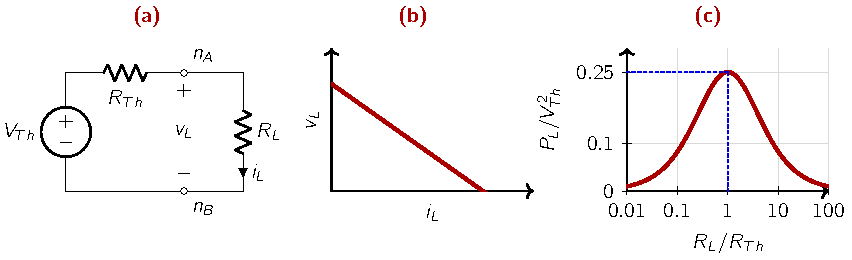
\includegraphics[width=\textwidth]{figure/ch02/fig02-06.pdf}
%     \caption{Maximum power transfer theorem.}
%     \label{fig:02-06}
% \end{figure}

% \begin{boxedstuff}
%     \begin{problem}
%         Prove the statements in Eq.~\ref{eq:02-25}. (\textit{Hint:} Use the first order condition for maximization of a continuous function.)
%     \end{problem}
% \end{boxedstuff}

% \subsection{RC, RL, and RLC Circuits}
% Unlike resistors, that neitther remember the past values of its votlage or current, capacitors and indutors retain memory of the past current and past voltage, respectively. This can be easily seen from their respective voltage-current relationships given by Eq.~\ref{eq:02-03} and Eq.~\ref{eq:02-07}, respectively. 

% \noindent\textbf{Capacitor:}
% \begin{equation}
%     i_C = C \frac{dv_C}{dt} \implies v_C\left(t\right) = \frac{1}{C}\int_{0}^{t} i_C\left(\tau\right) d\tau + v_C\left(0\right)
%     \label{eq:02-26}
% \end{equation} 
% The instantaneous voltage across a capacitor contains some information about the past history the current that has flown through the capacitor. This voltage $v_C\left(t\right)$ is determined by the charge on the capacitor at time $t$. Note, that the voltage across the capacitor cannot change instantaneously, as this would require an infinite current to flow through the capacitor. Theoretically, however, an impulse (Dirac delta function) current applied to the capacutor can produce instantaneous change in the capacitor's voltage.

% \noindent\textbf{Inductor:}
% \begin{equation}
%     v_L = L \frac{di_L}{dt} \implies i_L\left(t\right) = \frac{1}{L}\int_{0}^{t} v_L\left(\tau\right) d\tau + i_L\left(0\right)
%     \label{eq:02-27}
% \end{equation}
% Similarly, the instantaneous current through the inductor contains some information about the history of voltage applied across the inductor. Current through an inductor cannot change instantaneously, as this would require an infinite voltage to be applied across the inductor. An impulse voltage applied to the inductor can produce instantaneous change in the inductor's current.

% \noindent\textbf{RC Circuit.} Consider a simple RC circuit shown in Figure~\ref{fig:02-07a}. We can write Kirchoff's voltage law for the circuit as follows,
% \begin{equation}
%     RC \frac{d v_C}{dt} + v_C = V_s \implies v_C(t) = e^{-t/RC} \left[ v_{C}(0) + \int_0^t \frac{1}{RC} e^{\tau/RC} V_s(\tau)\, d\tau \right]
%     \label{eq:02-28}
% \end{equation}
% The above euqation gives the general solution for the voltage across the capactior. We can derive all other variables of interest from $v_C$. The response to an impulse input, step input, sinusoidal input, or any arbitrary $V_s$ can be computed using the above equation. The response for a step input obtained using a fixed sources and a swtich is given in Figure~\ref{fig:02-07a}. $RC$ is the time constant of the circuit, and is a measure of how fast the capacitor charges or discharges and it has the units of time.

% \begin{figure}[t]
%     \centering
%     \begin{subfigure}{0.48\textwidth}
%         \centering
%         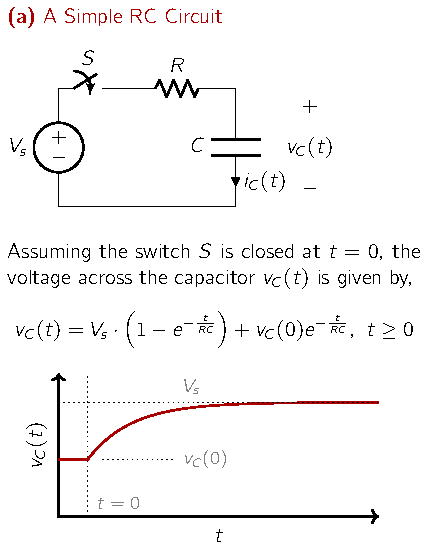
\includegraphics[width=\textwidth]{figure/ch02/fig02-07a.pdf}
%         \caption{Ideal voltage source}
%         \label{fig:02-07a}
%     \end{subfigure}
%     \hfill
%     \begin{subfigure}{0.48\textwidth}
%         \centering
%         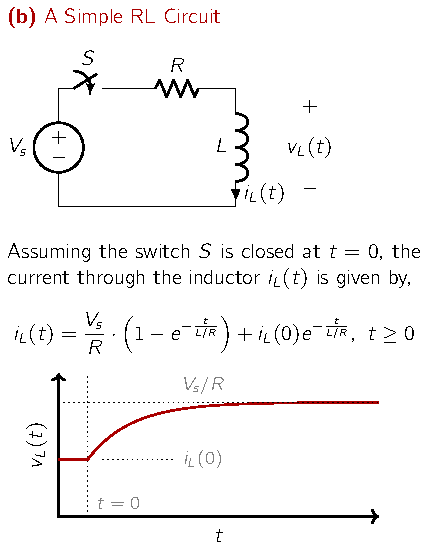
\includegraphics[width=\textwidth]{figure/ch02/fig02-07b.pdf}
%         \caption{Practical voltage source with a load}
%         \label{fig:02-07b}
%     \end{subfigure}
%     \caption{Simple RC and RL circuits and their transient responses.}
%     \label{fig:02-07}
% \end{figure}

% Using Laplace transform to analyze the circuit, we can write the following expression for the voltage across the capacitor,
% \begin{equation}
%     V_C(s) = \frac{1}{sRC + 1} V_s(s) + \frac{v_C(0)}{sRC + 1}
%     \label{eq:02-29}
% \end{equation}
% $V_C(s)$ and $V_s(s)$ are the Laplace transforms of $v_C(t)$ and $V_s(t)$. Replacing $s = j\omega$ will give us the frequency response of the system with $V_C(s)$ as the output and $V_s(s)$ as the input.

% \noindent\textbf{RL Circuit.} Consider a simple RL circuit shown in Figure~\ref{fig:02-07b}. Kirchoff's voltage law for the circuit is as follows,
% \begin{equation}
%     \frac{L}{R} \frac{di_L}{dt} + i_L = \frac{1}{R}V_s \implies i_L(t) = e^{-t/L} \left[ i_{L}(0) + \int_0^t \frac{1}{L} e^{\tau/L} V_s(\tau)\, d\tau \right]
%     \label{eq:02-30}
% \end{equation}
% The above euqation gives the general solution for the current through the inductor. The response to an impulse input, step input, sinusoidal input, or any arbitrary $V_s$ can be computed using the above equation. The response for a step input obtained using a fixed sources and a swtich is given in Figure~\ref{fig:02-07a}. $\frac{L}{R}$ is the time constant of the circuit, and is a measure of how fast the current through the inductor can chamge; it has the units of time.

% Similarly, applying the Laplace transform, we have,
% \begin{equation}
%     I_L(s) = \frac{1}{sL + R} V_s(s) + \frac{i_L(0)}{sL + R}
%     \label{eq:02-31}
% \end{equation}

% \noindent\textbf{RLC Circuit.} Consider a simple series RLC circuit shown in Figure~\ref{fig:02-08}. Kirchoff's voltage law for the circuit is as follows,
% \begin{equation}
%     LC\frac{d^2 v_C}{dt^2} + RC \frac{d v_C}{dt} + v_C = V_s 
%     \label{eq:02-32}
% \end{equation}
% \begin{figure}[t]
%     \centering
%     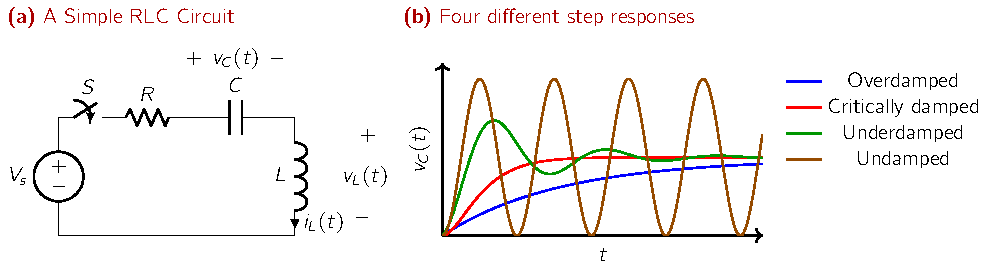
\includegraphics[width=\textwidth]{figure/ch02/fig02-08.pdf}
%     \caption{A simple RLC circuit and the different respones of the circuit when the switch $S$ is closed at time $t = 0$, with  zero initial capacitor voltage and inductor current whent .}
%     \label{fig:02-08}
% \end{figure}
% The response of the circuit when the switch is closed at $t=0$ is qualitatively different depending on the values of $R$, $L$ and $C$. This is better understood in the Laplace domain. The Laplace transform of the response $v_c(t)$ is given by,
% \begin{equation}
%     V_C(s) = \frac{V_s(s)}{LCs^2 + RCs + 1} + v_C(0)\frac{C\left(Ls + R\right)}{LCs^2 + RCs + 1} + i_L(0)\frac{RC}{LCs^2 + RCs + 1}
%     \label{eq:02-33}
% \end{equation}
% Note that $i_L(0) = \frac{d v_C}{dt}(0)$. The denominator of the above equation is a second order polynomial in $s$, and thus the response of the circuit will depend on the roots of the polynomial. The four different responses are shown in Figure~\ref{fig:02-08}.

% \subsection{Steady State Sinusoidal Analysis}
% The previous subsection looked at the transient response of the some simple circuits involving $R$, $L$, and $C$. However, we are often interested in the steady state response of these circuits to sinussoidal excitations. This is because sinusoisal signals are eigenfunctions of linear systems, such as the linear circuits we have discussed so far. With sinusoidal excitations, all currents and voltages in the circuit will also be sinusoidal with the same frequency as the input excitations, althought with different amplitudes and phases. Complex numbers are used to in this analysis as for compact representation of ampltiude and phase of signals. 

% For steady state frequency analysis for circuits involving $R$, $L$, and $C$, we extend the idea of resistance to impedance. Fourier transforms provide a natural way to analyze the steady state response of linear circuits to sinusoidal excitations. We first recast the voltage-current relationships of the circuit elements in the Fourier domain. 
% \begin{equation}
%     \begin{split}
%         \textbf{Resistor:} \quad & v_R = R \, i_R \implies V_R\left(j\omega\right) = R \cdot I_R\left(j\omega\right)\\
%         \textbf{Capacitor:} \quad & i_C = C\frac{d v_C}{dt} \, \implies V_C\left(j\omega\right) = \frac{1}{j\omega C} \cdot I\left(j\omega\right)\\
%         \textbf{Inductor:} \quad & v_L = L \frac{d i_L}{dt} \implies V_L\left(j\omega\right) = j\omega L \cdot I_L\left(j \omega \right)
%     \end{split}
%     \label{eq:02-34}
% \end{equation}

% The Fourier transformed voltage-current relationships of the circuit elements look like Ohms law, with the concept of resistance extended to impedance. The impedance of a capacitor and inductor defined as the are defined as the ratio of the Fourier transformed voltage to the Fourier transformed current. They are functions of the frequency of the voltage/current. The impedance of a resistor, capacitor, and inductor are given by,
% \begin{equation}
%     \begin{split}
%         \textbf{Resistor:} \quad & Z_R = R\\
%         \textbf{Capacitor:} \quad & Z_C = \frac{1}{j\omega C}\\
%         \textbf{Inductor:} \quad & Z_L = j\omega L
%     \end{split}
%     \label{eq:02-35}
% \end{equation}

% \noindent\textbf{Equivalent Impedance.} The equivalent impedance of a circuit with impedances $Z_1, Z_2, \cdots Z_n$ in series is given by $Z_{eq} = Z_1 + Z_2 + \cdots + Z_n$. When the impedances $Z_1, Z_2, \cdots Z_n$ are in parallel, the equivalent impedances is given by $\frac{1}{Z_{eq}} = \frac{1}{Z_1} + \frac{1}{Z_2} + \cdots + \frac{1}{Z_n}$.

% \noindent\textbf{Amplitude and phase modification by an impedance.} If a sinusoidal current excitation $i\left(t\right) = I_o \sin\left(\omega t\right)$ is passed through an impednace $Z$. Then the voltage across the impedance is given by,
% \begin{equation}
%     v\left(t\right) = \vert Z \vert I_o \sin\left(\omega t + \arg Z \right)
%     \label{eq:02-36}
% \end{equation}
% The amplitude of the sinusoidal voltage is $\vert Z \vert I_o$, and the phase of the sinusoidal voltage is $\arg Z$, with respect to the current $i\left(t\right)$. 

% \subsection{Exercise}
% \vspace{-0.5cm}
% \begin{center}
%     \rule{\textwidth}{1pt}
% \end{center}

% \begin{enumerate}
%     \item Plot the current across a resistor $R = 10\Omega$, capacitor $C = 5\mu F$, and inductor $L = 2mH$ for the following voltage inputs.
%     \begin{figure}[h]
%         \centering
%         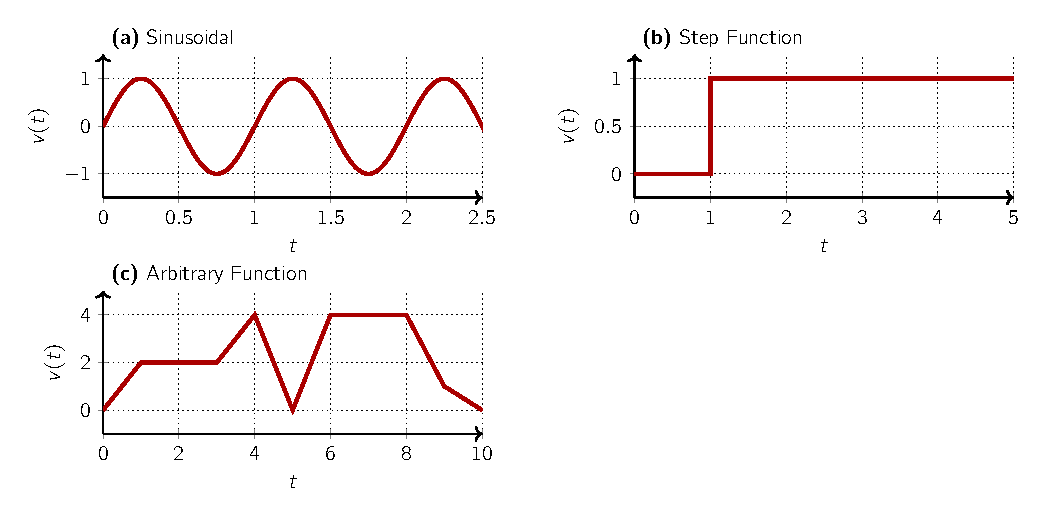
\includegraphics[width=\textwidth]{figure/ch02/ex02-01.pdf}
%         \caption{[Exercise 1] Voltage inputs applied to a resistor, capacitor, or an inductor. The units of voltage are in volts, and the time is in seconds.}
%         \label{fig:ex02-01}
%     \end{figure}
    
%     \item Find the Thevenin and Norton equivalent circuits of the following circuits (Figure~\ref{fig:ex02-02}). Note that one of the problems has a dependent source. Dependent sourcrs are voltage or current sources (diamond shaped elements), whose voltage or current, respectively, depend on the voltage or current across another element in the circuit.
%     \begin{figure}[h]
%         \centering
%         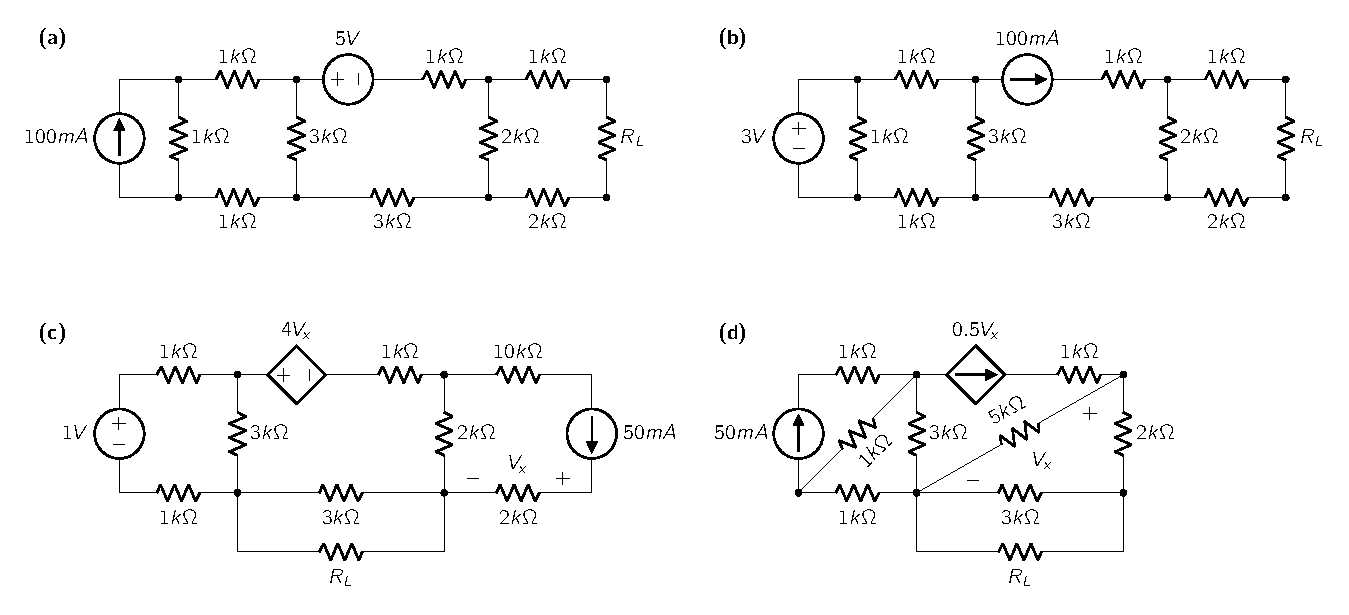
\includegraphics[width=\textwidth]{figure/ch02/ex02-02.pdf}
%         \caption{[Exercise 2] Find the equivalent impedance of the circuit.}
%         \label{fig:ex02-02}
%     \end{figure}
    
%     \item A certain red LED has a maximum current rating of $35 mA$, and if this value is exceeded, overheating and catastrophic failure will result. The resistance of the LED is a nonlinear function of its current, but the manufacturer warrants a minimum resistance of $47 \Omega$ and a maximum resistance of $117 \Omega$. Only $9 V$ batteries are available to power the LED. Design a suitable circuit to deliver the maximum power possible to the LED without damaging it. Use only combinations of the standard resistor values. (\textit{This problem is from Engineering Circuit Analysis by Hayt Jr. et al.})
    
%     \item The load resistor in Figure~\ref{fig:ex02-03} can safely dissipate up to $1W$ before overheating and bursting into flame. The lamp can be treated as a $10.6\Omega$ resistor if less than $1A$ flows through it and a $15\Omega$ resistor if more than $1A$ flows through it. What is the maximum permissible value of $I_s$? Verify your answer with an appropriate computer simulation. (\textit{This problem is from Engineering Circuit Analysis by Hayt Jr. et al.})
%     \begin{figure}[h]
%         \centering
%         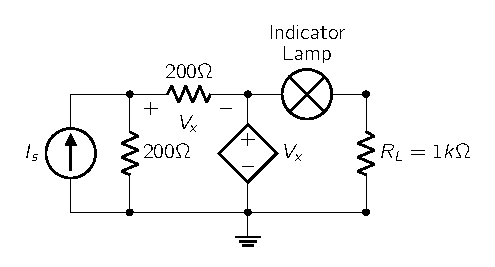
\includegraphics[width=0.65\textwidth]{figure/ch02/ex02-03.pdf}
%         \caption{[Exercise 4]Find the equivalent impedance of the circuit.}
%         \label{fig:ex02-03}
%     \end{figure}
    
%     \item In the following circuit (Figure~\ref{fig:ex02-04}), find the voltage across the capacitors $C_1$ and $C_2$. The single pole double throw swtich $S$ is connect to the top terminal before time $t=0$. At time $t=0$, swtich is flipped to the bottom terminal.  Assume that the before time $t=0$, the voltage across the capacitor $C_2$, $v_{C2} = 1V$. Draw the plot of the voltage across the capcitors $C_1$ and $C_2$ as function of time.
%     \begin{figure}[h]
%         \centering
%         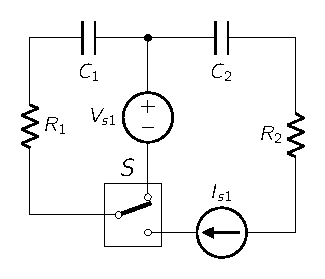
\includegraphics[width=0.35\textwidth]{figure/ch02/ex02-04.pdf}
%         \caption{[Exercise 5]Find the equivalent impedance of the circuit.}
%         \label{fig:ex02-04}
%     \end{figure}
    
%     \item Figure~\ref{fig:ex02-05} shows a voltage divider circuit with a sinusoidal voltage source $V_s\left(t\right) = 10 \sin\left(1000\pi t\right)$. The impedane $Z_1 = 3 + j4 \Omega$. What should the impedance $Z_2$ be if the the voltage across $Z_2$ has one-fourth the amplitude of $V_s$ and with a phase difference of $45\deg$?
%     \begin{figure}[h]
%         \centering
%         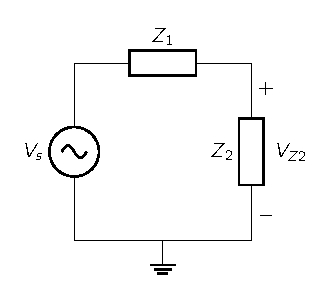
\includegraphics[width=0.35\textwidth]{figure/ch02/ex02-05.pdf}
%         \caption{[Exercise 5]Find the equivalent impedance of the circuit.}
%         \label{fig:ex02-05}
%     \end{figure}
% \end{enumerate}